\chapter{Web Server}
\label{sec:webserver}

\author{Nico Leidenfrost}
%
To make a web application accessible to a user, there needs to be a web server which serves the files to the web browser of the user. In the case of GRAMOC, NGINX was chosen to be used as a web server \autocite{nginx}.

A web server is a server dedicated to provide information, web sites or web applications. To achieve this goal the web server first transmits the files needed to run the web application and then sends information whenever it is requested.

\section{Apache}
Apache HTTP Server was first launched in 1995 \autocite{apache}. It gained a lot of popularity very quickly and since April 1996 it is the most used web server of active websites. Apache's approach on how to handle incoming connections is quite simple: for each connection there is one thread. This can lead to problems when a lot of clients are trying to connect to the server at the same time. Apache consists of a core module and many dynamically loadable modules. These modules provide various features like:

\begin{itemize}
    \item Support for various programming languages
    \item URL rewrite
    \item Proxy functionality
    \item SSL support
    \item Authentication utilities
\end{itemize}

This module system gives Apache a lot of power in terms of flexibility, because there is no need to use other systems as Apache itself is most often able to provide these features.

\section{NGINX}
NGINX, pronounced \textit{engine x}, is a lightweight web server that was initially created to solve the \textit{c10K} problem. The goal of this challenge was to create a web server that is able to handle ten thousand concurrent client connections at once. To achieve this goal, the main difference between NGINX and its competitors is that NGINX handles client connections asynchronously instead of synchronously. NGINX is also event driven and single threaded. This means that there is only one thread running and not one thread per connection. In GRAMOC, NGINX is used to provide only the core features of a web server, namely providing static web application content and basic routing between the web server and the Node.js server. Any other functionality will be passed to components that can handle the specific tasks. NGINX was chosen over Apache because of its lightweight design and speed. This is mainly achieved through passing on tasks to other programs and not trying to handle everything on its own like Apache does.

\section{Apache vs NGINX}
According to Upguard, a cyber security company, NGINX is about 4.2 times faster than Apache \autocite{UpguardAvN}. The main reason for this is the single threaded, asynchronous approach of NGINX.
Apache however contains a much larger feature set and better support, because of the fact that Apache is a lot older than NGINX. The smaller feature set of NGINX can be seen as a disadvantage, but also as an advantage. Less features are usually a clear disadvantage, but on the other hand if there are less features available, the system is much more lightweight. That is one of the main reasons why NGINX was chosen in GRAMOC. Due to this lightweight design, NGINX can operate also on systems with less computing power, like the Raspberry Pi that is used in GRAMOC.

In terms of popularity Apache is at the time of writing twice as much used in web server development as NGINX. These figures originate from the \textit{February 2018 Web Server Survey} conducted by Netcraft and are shown in figure \vref{fig:netcraft_survey} \autocite{netcraft_survey}.

\begin{figure}[h]
    \centering
    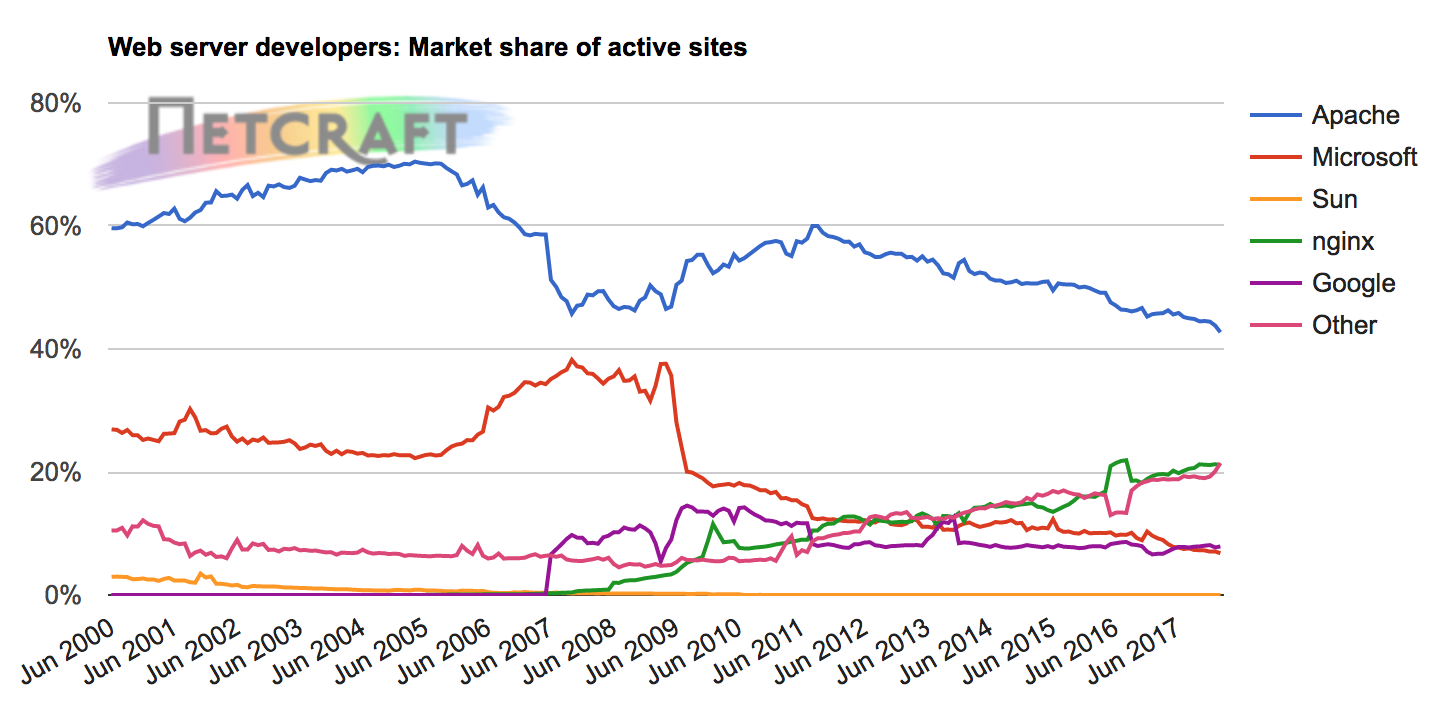
\includegraphics[width=15cm,keepaspectratio]{netcraft_survey}
    \caption{Survey results about most used web servers in currently active websites}
    \label{fig:netcraft_survey}
\end{figure}

These results show that Apache is still the number one web server with 42.72 percent market share. Number two with 21.13 percent is NGINX. The trend shows that NGINX is gaining more and more popularity as Apache slowly looses its market share. Below these two main competitors there is Google's in house developed web server, which they use for their own services, and Microsoft's IIS.

\section{Node.js}
\label{sec:nodejs}
Node.js is an asynchronous, event driven JavaScript runtime, designed to build network applications \autocite{Node}. The built-in HTTP module can be used to create a web server based on Node.js. This module is used to utilise communication over the HTTP protocol. In terms of GRAMOC the sensor data is received via a UDP connection and then transmitted over HTTP to the web application. Therefore, the main task of the Node.js server is to receive data which is emitted by the Filtering and Preprocessing Layer (FAPS) and forward it, to the web application via WebSockets implemented through the \textit{socket.io} library \autocite{socketio}. In order to use socket.io the HTTP module in combination with the express framework must be used.

To implement an API (Application Programming Interface) to retrieve historical data, also Node.js was used. The actual framework that was used to implement the API is called \textit{Express} (see below section \vref{sec:express}).

\section{Express}
\label{sec:express}
Express is a minimal and flexible web application framework to be used with Node.js. It is build on top of the HTTP module provided by Node.js. Handling basic routing tasks and creating powerful APIs (Application Programming Interfaces) are the main tasks of the Express framework. Sometimes Express is mistaken to be a web server on itself, but it is just a layer on top of a web server. Express was used to create the REST API used in GRAMOC (see below section \vref{sec:restapi}).

\section{socket.io}
\label{sec:socketio}
socket.io is a JavsScript library that implements real-time communication via WebSockets. This library was selected to be used within this project, because it aims to make real-time applications possible in every browser. Socket.io is available for both Node.js and Vue.js. The socket.io framework works well within GRAMOC, because GRAMOC also aims to deliver sensor data in real-time.

\section{REST API}
\label{sec:restapi}
GRAMOC also saves the incoming sensor data beside plotting it. This data is especially useful to create statistics or if a user wants to inspect the sensor data of a certain point of time. How the data is saved is further explained in chapter \vref{ch:faps-save}. To make the stored sensor data available to users, a REST API was implemented.
REST means \textit{Representational State Transfer}, which is an architectural style. To call an API RESTful it needs to satisfy a number of constraints \autocite{rest}:

\begin{itemize}
    \item Client-Server
    \item Stateless
    \item Cache
    \item Uniform Interface
    \item Layered System
    \item Code-On-Demand
\end{itemize}

\subsection{Client-Server}
REST features a client-server model, like many other web based architectures. The main concept of this model is that two clients can not talk directly to each other. Every client needs to communicate with a server. If network units need to communicate with each other, then every unit must implement a client and a server. This separation of client and server can lead to better scalability of each component, as they are developed independently.

\subsection{Stateless}
A stateless system can not store data from clients to use this data in future requests. Each request must contain enough information, so that the server is able to send an appropriate response. This constraint leads also to improved performance as the server does not need to store any contextual data about clients and is therefore able to process multiple requests faster.

\subsection{Cache}
A response must be explicitly marked as cacheable or non-cacheable. If a response is marked as cachable, it can be reused for future equivalent requests. This is useful if such cached information can be reused at least one time, because then the client can simply use the cached data instead of sending a new request to the server every time.

\subsection{Uniform Interface}
A REST API should have a standardised uniform interface in order to maintain the simplicity of interactions. A resource in a system should only have one logical URI.

\subsection{Layered System}
In a layered system, every component can access only the layer next to it. This removes a lot of complexity from the system, as a component just needs to interact with its neighbours.

\subsection{Code-On-Demand}
The last constraint within the REST architecture is the Code-On-Demand constraint which is only optional. It allows an API to send executable code to the clients to extend their set of features. This is used to create simple clients which can be dynamically extended after deployment.

\subsection{Implementation}
In the GRAMOC REST API are only GET routes, as there is no need to change or modify data. The available routes are listed in table \vref{tab:get_routes}.

\begin{table}[H]
    \centering
    \begin{tabular}{| l | l |}
    \hline
    \textbf{Route} & \textbf{Response} \\ \hline
    /files & returns a list of files within the data directory \\ \hline
    /files/:file/data & returns the data of each dataset inside a file \\ \hline
    /files/:file/datasets & returns a list of datasets stored inside a file \\ \hline
    /files/:file/datasets/:id & returns the data of a specific dataset \\
    \hline
    \end{tabular}
    \caption{GET request routes of the REST API used in GRAMOC}
    \label{tab:get_routes}
\end{table}

The files are all stored in a specific directory from which the API can read. Inside these files there are datasets, which represent time points. With this structure it is possible to request the data from a specific timespan.

\subsubsection{Pagination}
Due to the large amounts of data, one request took longer to process than the timeout of the web browser allowed. This problem was solved by using pagination. Pagination is a technique to split the whole data from one big request into more smaller requests. These requests can be processed much faster and therefore a response can be send in time. To use pagination a query string with the parameters \textit{limit} and \textit{page} must be provided. The limit indicates the maximum amount of data which can be transmitted by one response. The page parameter specifies the offset of the data which has to be send. To check if another page is available, every response contains a field \textit{has\_more}.
